\chapter{Braking System Calculations}
\label{appx:braking-calcs}

\section{Main Shaft Calculations}
\label{calcs:main_braking_shaft}

\begin{figure}[H]
    \centering
    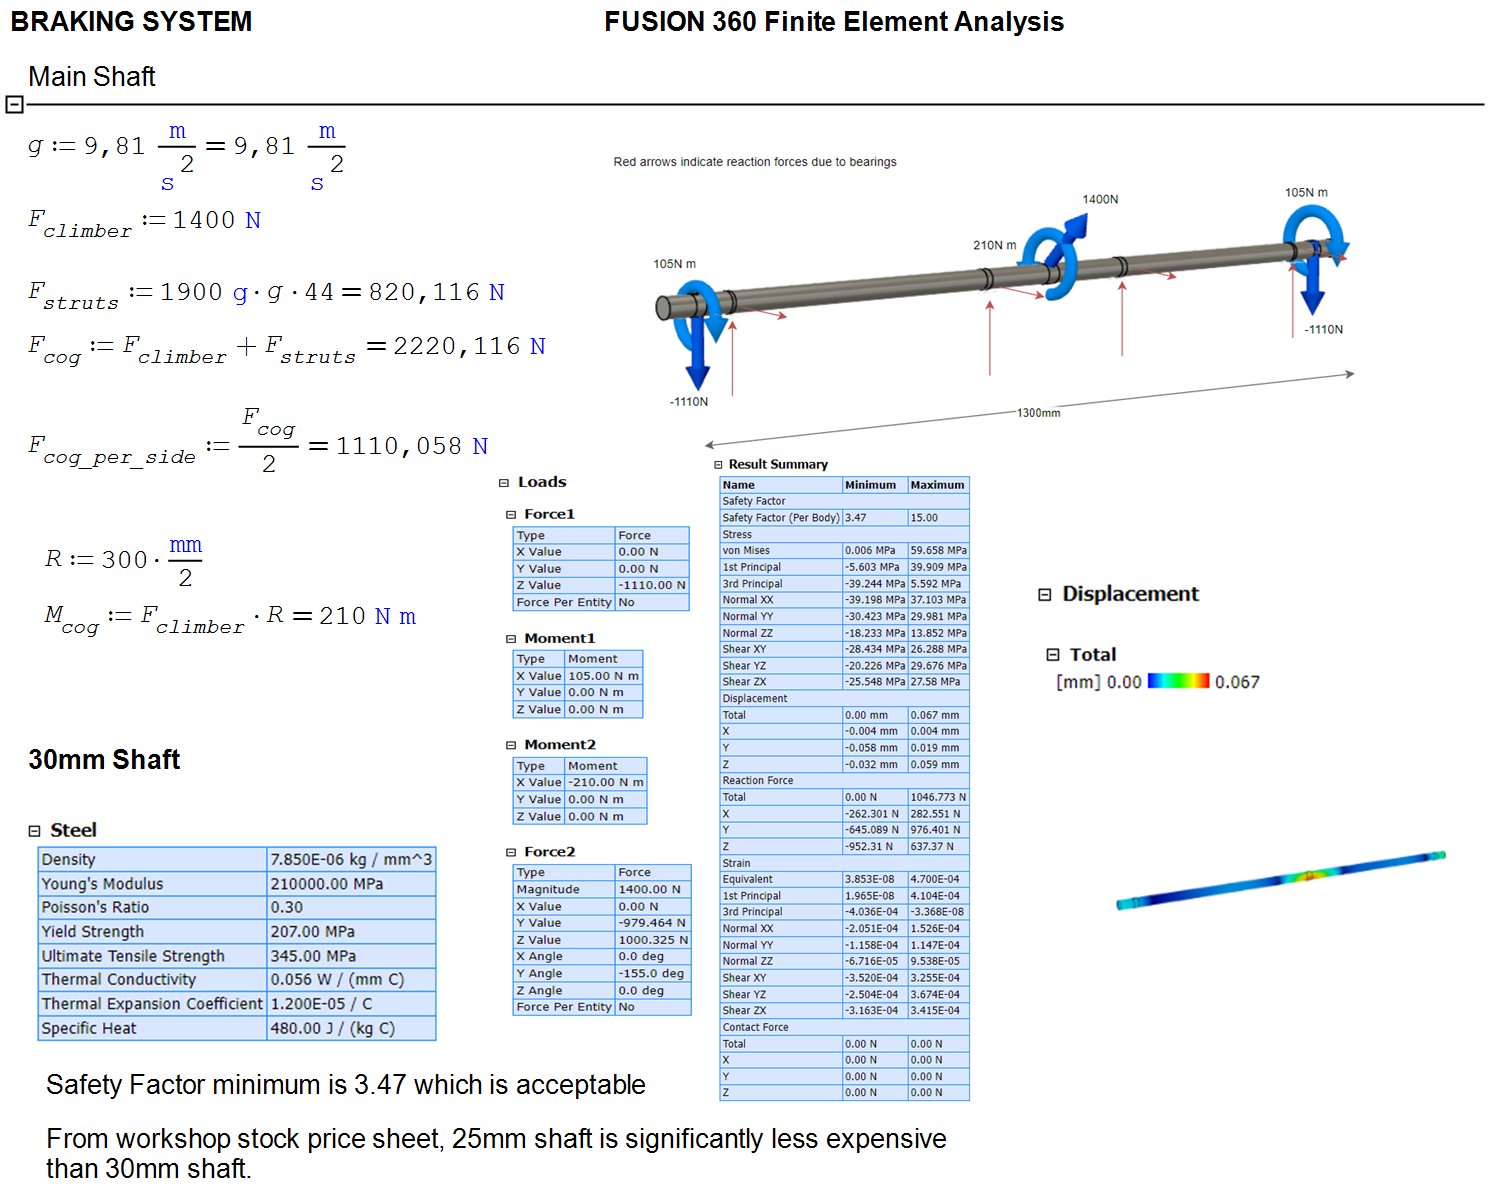
\includegraphics[width=0.9\linewidth]{chaps-append/calcs/main_shaft_calcs1.png}
\end{figure}

\begin{figure}[H]
    \centering
    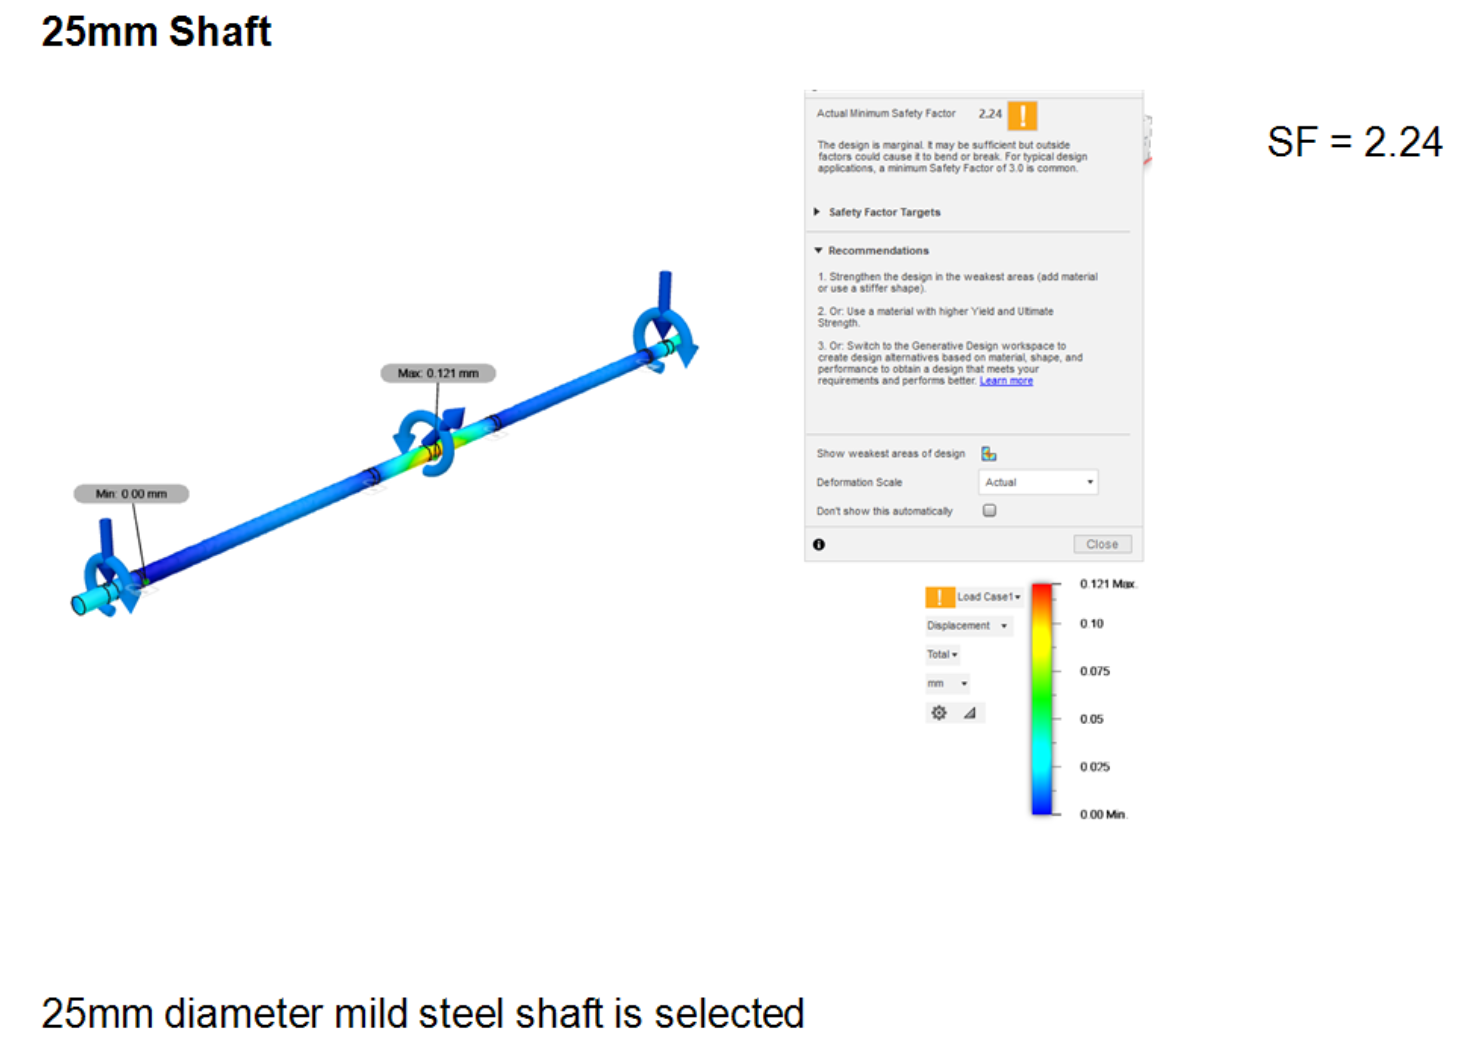
\includegraphics[width=0.7\linewidth]{chaps-append/calcs/main_shaft_calcs_2.png}
\end{figure}

\section{Brackets and Bearings Calculations}
\label{calcs:brackets_bearings}

\subsection*{Laser Cut Brackets}

\begin{figure}[H]
    \centering
    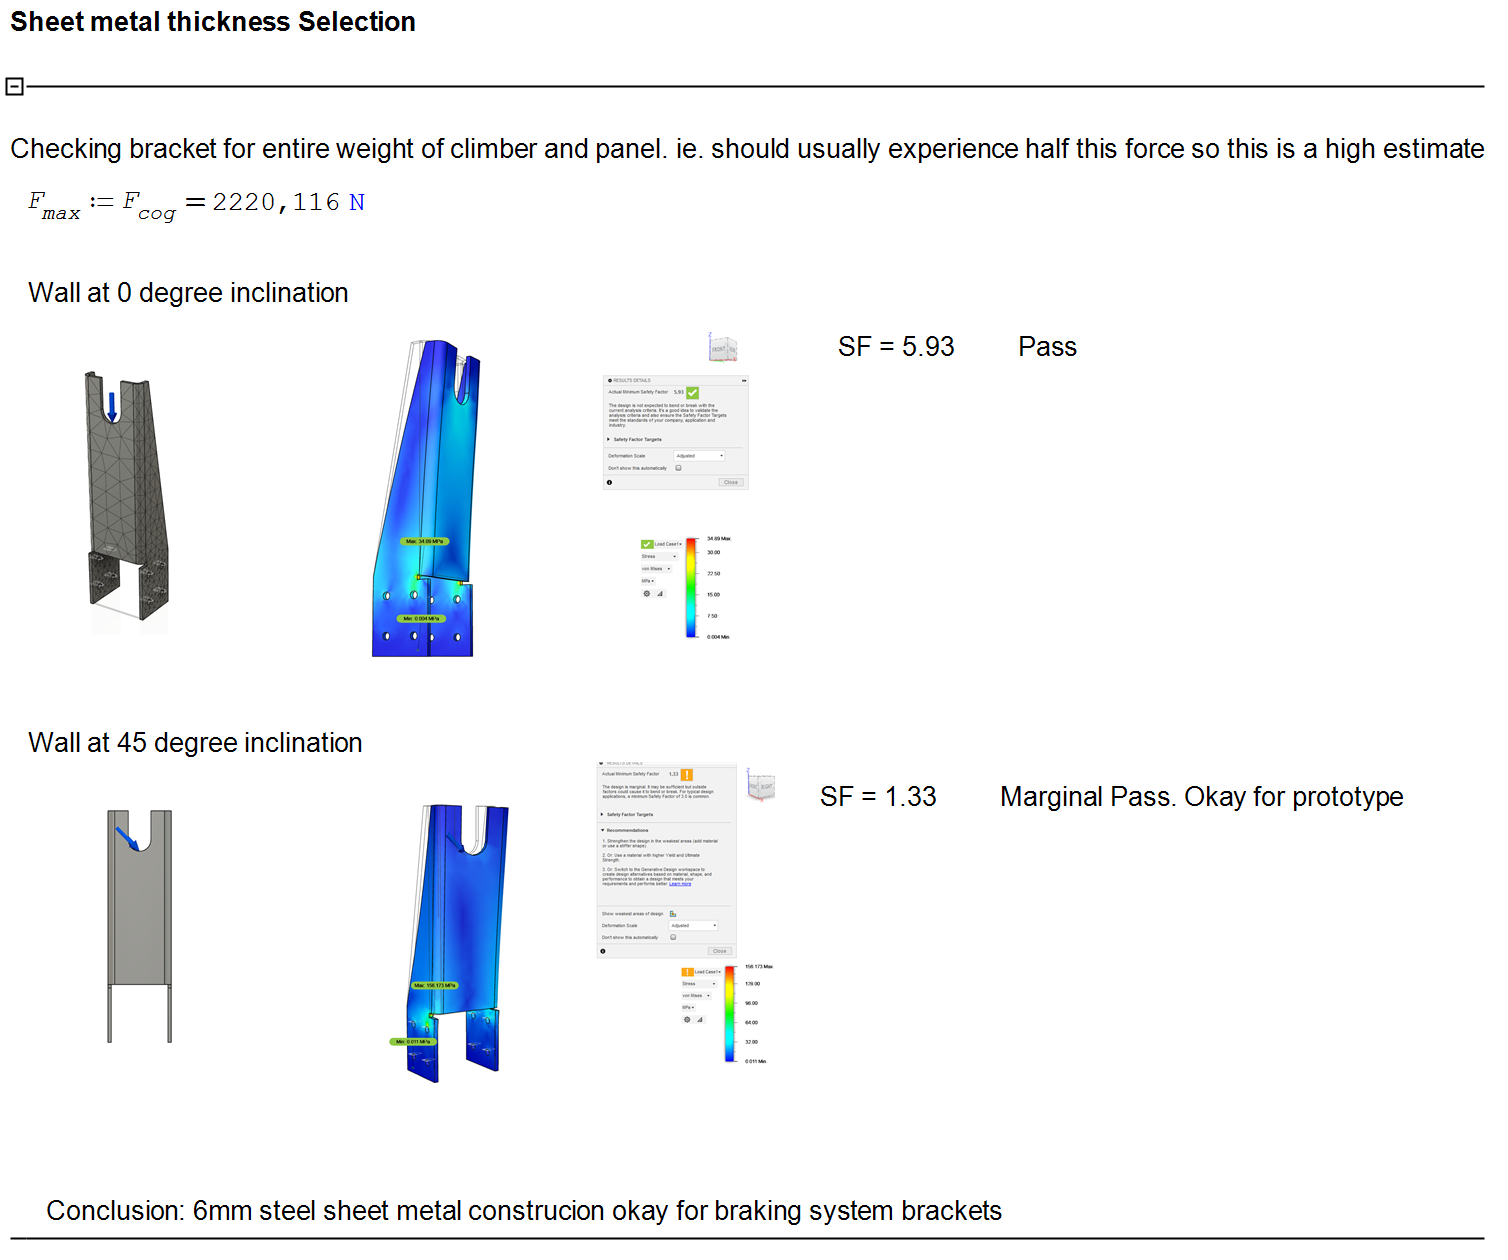
\includegraphics[width=1\linewidth]{chaps-append/calcs/FEM_brackets.png}
\end{figure}

\subsection*{Main Shaft Bearing Verification}

Assuming the bearings transfer all the force from the shaft to the brackets, the maximum force is calculated as:

\[
F_{\text{max}} = 2220\ \text{N}
\]

Using a \textbf{Koyo UCF205 Flange unit bearing} with a basic load rating of \( C_{0r} = 7.85\ \text{kN} \), the bearing can safely handle the applied load.

\section{Motor and Belt Drive System Calculations}
\label{calcs:motor_belt}

\subsection*{Mechanical Losses in Rotating System}

There is a significant amount of torque lost due to friction in the bearings and panels sliding through aluminum channels. Accounting for these frictional losses reduces the torque needed to brake the system and allows for a simpler motor and pulley system.

First, calculate the gravitational force due to the wood panels:

\[
F_{\text{woodPanels}} = N_{\text{panels}} \times m_{\text{panel}} \times g = 41 \times 2\ \text{kg} \times 9.81\ \text{m/s}^2 = 803.22\ \text{N}
\]

Where:
\begin{itemize}
    \item \( N_{\text{panels}} = 41 \) is the number of panels.
    \item \( m_{\text{panel}} = 2\ \text{kg} \) is the mass of each panel.
    \item \( g = 9.81\ \text{m/s}^2 \) is the acceleration due to gravity.
\end{itemize}

Next, consider the weight of the climber (assuming a maximum climber mass of 90\,kg):

\[
F_{\text{climber\_low}} = m_{\text{climber\_low}} \times g = 90\ \text{kg} \times 9.81\ \text{m/s}^2 = 882.9\ \text{N}
\]

The torque due to the climber's weight is:

\[
M_{\text{climber\_low}} = F_{\text{climber\_low}} \times r = 882.9\ \text{N} \times 1\ \text{m} = 882.9\ \text{Nm}
\]

Assuming rotational equilibrium, the normal force on each wall due to the climber is:

\[
F_{\text{N\_W}} = \frac{M_{\text{climber\_low}}}{2 \times L} = \frac{882.9\ \text{Nm}}{2 \times 0.85\ \text{m}} = 519.35\ \text{N}
\]

Where \( L = 0.85\ \text{m} \) is the horizontal distance from the pivot to the point of contact.

The coefficient of dynamic friction between aluminum and nylon is:

\[
\mu_{\text{alu\_nylon}} = 0.25
\]

The frictional force at one contact point is:

\[
F_{\text{f,single}} = F_{\text{N\_W}} \times \mu_{\text{alu\_nylon}} = 519.35\ \text{N} \times 0.25 = 129.84\ \text{N}
\]

The total frictional force due to all four contact points is:

\[
F_{\text{f}} = 4 \times F_{\text{f,single}} = 4 \times 129.84\ \text{N} = 519.35\ \text{N}
\]

The braking torque produced by this friction is:

\[
T_{\text{friction}} = F_{\text{f}} \times \frac{D}{2}
\]

Assuming the diameter \( D \) is such that \( T_{\text{friction}} = 64.92\ \text{Nm} \), we proceed with this value.

The torque required on the shaft to overcome the climber's weight, accounting for friction, is:

\[
T_{\text{shaft}} = F_{\text{climber\_low}} \times \frac{D}{2} - T_{\text{friction}} = 45.44\ \text{Nm}
\]

This reduced torque requirement allows for the selection of a less powerful motor, optimizing cost and efficiency.

\subsection*{Torque Reduction Ratio Calculation}

The required torque at the shaft is:

\[
T_{\text{shaft}} = 45.44\ \text{Nm}
\]

The motor's continuous torque is:

\[
T_{\text{motor}} = 10\ \text{Nm}
\]

Therefore, the necessary gear reduction ratio is:

\[
R = \frac{T_{\text{shaft}}}{T_{\text{motor}}} = \frac{45.44\ \text{Nm}}{10\ \text{Nm}} = 4.544
\]

A gear reduction ratio of approximately 5:1 is required. This justifies the selection of the 90-tooth to 18-tooth pulley system, providing the needed gear ratio.

\subsection*{Motor Selection}

Based on the torque and speed requirements calculated, the motor must provide a continuous torque of at least 10\,Nm and operate at speeds up to 1000\,rpm. The \textbf{MiGE 130ST-M10010} motor was selected due to its specifications matching these requirements.

\paragraph{Motor Requirements}

- \textbf{Continuous torque required after gear reduction}:

\[
T_{\text{motor}} = \frac{T_{\text{shaft}}}{R} = \frac{45.44\ \text{Nm}}{5} = 9.09\ \text{Nm}
\]

- \textbf{Speed required at motor shaft}:

\[
n_{\text{motor}} = n_{\text{shaft}} \times R = 159\ \text{rpm} \times 5 = 795\ \text{rpm}
\]

\paragraph{Motor Specifications}

- \textbf{Continuous torque}: 10\,Nm
- \textbf{Rated speed}: 1000\,rpm

These specifications meet or exceed the calculated requirements, confirming the suitability of the MiGE 130ST-M10010 motor for this application.

\begin{figure}[H]
    \centering
    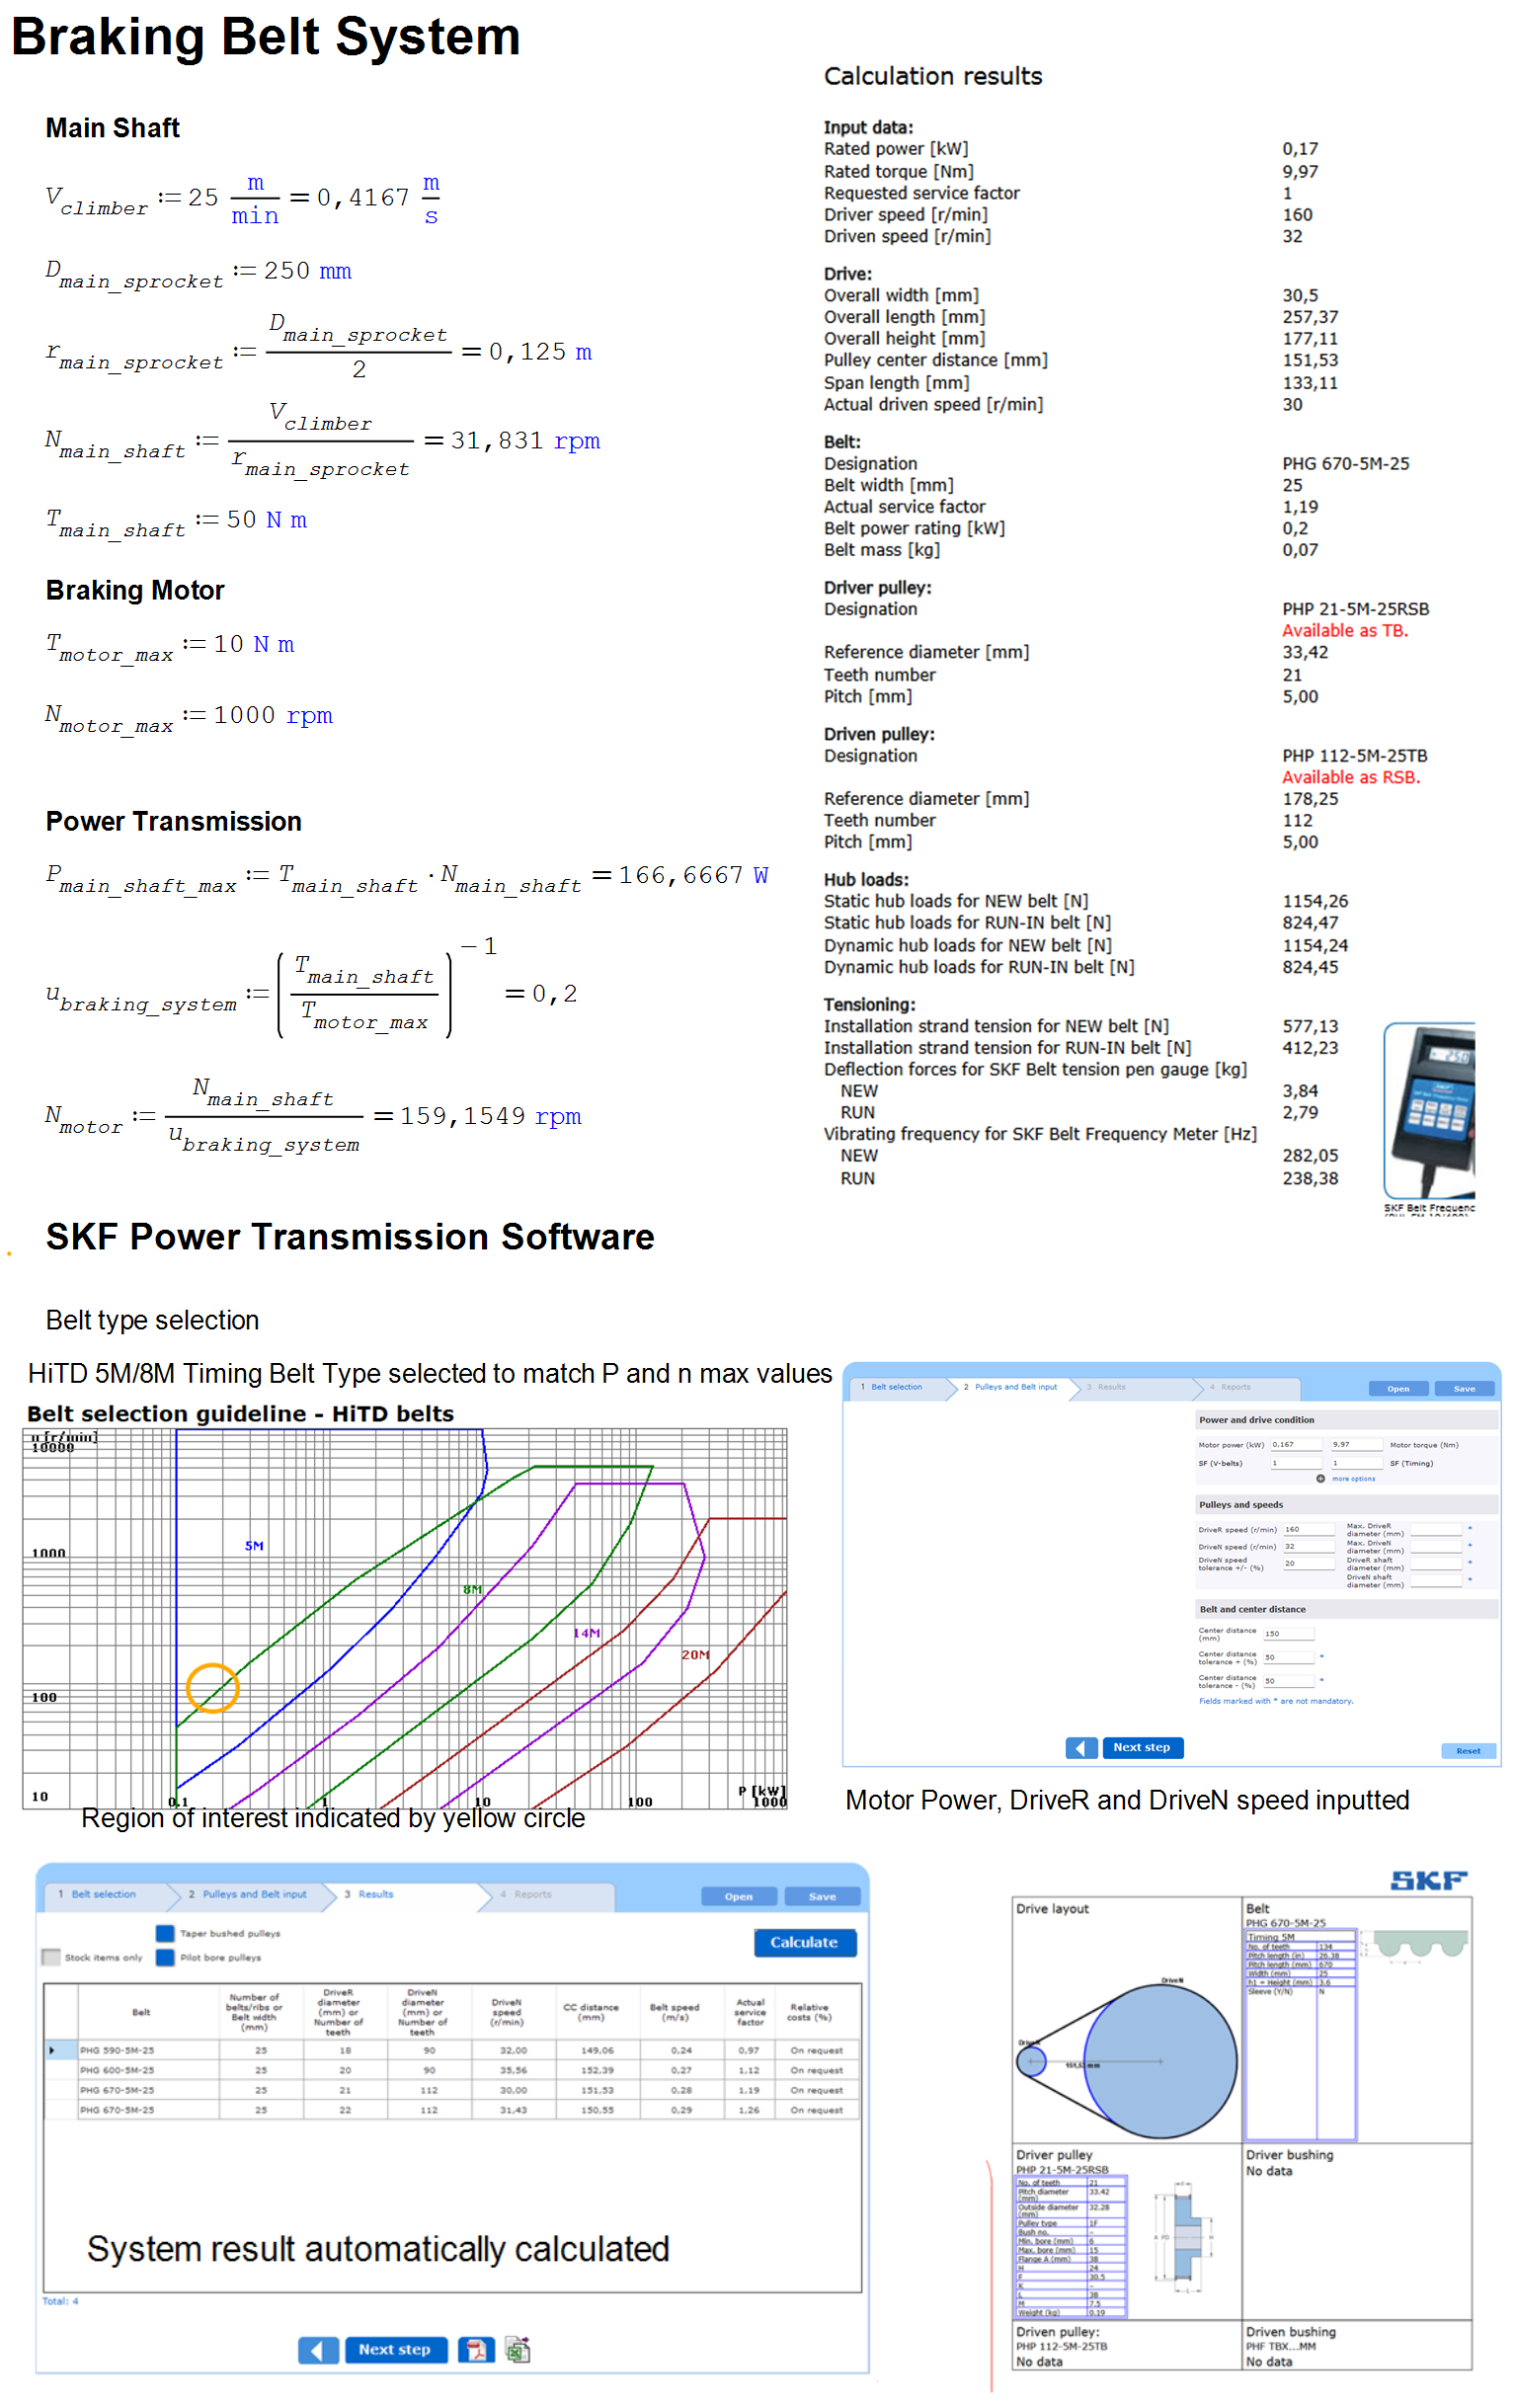
\includegraphics[width=1\linewidth]{chaps-append/calcs/belt_selection.png}
\end{figure}

\section{Braking Resistor Design}
\label{calcs:braking_resistor}

To determine the appropriate braking resistor, we calculate the voltage at the maximum motor speed using the voltage constant of the motor.

The voltage constant of the MiGE 130ST-M10010 motor is:

\[
K_v = 140\ \text{V/krpm}
\]

Assuming the maximum motor speed in this application is:

\[
n_{\text{max}} = 159\ \text{rpm}
\]

Converting rpm to krpm:

\[
n_{\text{max, krpm}} = \frac{159\ \text{rpm}}{1000} = 0.159\ \text{krpm}
\]

Calculating the maximum generated voltage:

\[
V_{\text{max\_speed}} = K_v \times n_{\text{max, krpm}} = 140\ \text{V/krpm} \times 0.159\ \text{krpm} = 22.26\ \text{V}
\]

The braking power remains:

\[
P_{\text{brake}} = P_{\text{gen}} \times 1.5 = 227.22\ \text{W}
\]

The current through the braking resistor is:

\[
I_{\text{brake}} = \frac{P_{\text{brake}}}{V_{\text{max\_speed}}} = \frac{227.22\ \text{W}}{22.26\ \text{V}} = 10.21\ \text{A}
\]

Finally, the braking resistor value is calculated as:

\[
R_{\text{brake}} = \frac{V_{\text{max\_speed}}}{I_{\text{brake}}} = \frac{22.26\ \text{V}}{10.21\ \text{A}} = 2.18\ \Omega
\]
